\documentclass{article}

\usepackage{tikz}

%--------------------------------------------------
%: math3d
\tikzset{math3d/.style={x={(-0.353cm,-0.353cm)},z={(0cm,1cm)},y={(1cm,0cm)}}}

%--------------------------------------------------
\begin{document}

\begin{center}
	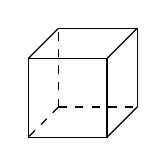
\begin{tikzpicture}
		\draw [dashed] (0,0,0) edge (1,0,0) edge (0,1,0) edge (0,0,1);
		\draw (1,0,0) -- (1,1,0);
		\draw  (1,1,0) -- (0,1,0) ; % face arriere
		\draw (0,0,1) -- (1,0,1) -- (1,1,1) -- (0,1,1) -- cycle; % face avant
		% aretes horizontales, de l'arriere vers l'avant
		\draw (1,0,0) -- (1,0,1);
		\draw (1,1,0) -- (1,1,1);
		\draw (0,1,0) -- (0,1,1);
	\end{tikzpicture}
\end{center}

\begin{center}
	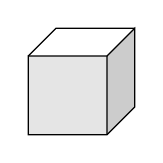
\begin{tikzpicture}[math3d]
		\coordinate (a) at (1,0,0);
		\coordinate (b) at (1,1,0);
		\coordinate (c) at (0,1,0);
		\coordinate (d) at (0,0,0);
		\coordinate (e) at (1,0,1);
		\coordinate (f) at (1,1,1);
		\coordinate (g) at (0,1,1);
		\coordinate (h) at (0,0,1);
		\fill[fill=white] (e) -- (f) -- (g) -- (h) -- cycle; % dessus
		\fill[fill=gray!20] (a) -- (b) -- (f) --(e) -- cycle; % avant
		\fill[fill=gray!40] (b) -- (c) -- (g)-- (f) -- cycle; % droite
		\draw (a) -- (e) -- (f) -- (g) -- (c) -- (b) -- cycle;
		\draw (e) -- (h) -- (g)  (b)--(f);
	\end{tikzpicture}
\end{center}

\begin{center}
	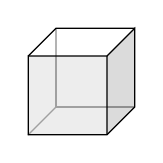
\begin{tikzpicture}[math3d]
		\coordinate (a) at (1,0,0);
		\coordinate (b) at (1,1,0);
		\coordinate (c) at (0,1,0);
		\coordinate (d) at (0,0,0);
		\coordinate (e) at (1,0,1);
		\coordinate (f) at (1,1,1);
		\coordinate (g) at (0,1,1);
		\coordinate (h) at (0,0,1);
		\draw (d) edge (a) edge (c) edge (h);
		% dessus
		\fill[fill=white, opacity=0.7] (e) -- (f) -- (g) -- (h) -- cycle;
		% avant
		\fill[fill=gray!20, opacity=0.7] (a) -- (b) -- (f) --(e) -- cycle;
		% droite
		\fill[fill=gray!40, opacity=0.7] (b) -- (c) -- (g)-- (f) -- cycle;
		\draw (a) -- (e) -- (f) -- (g) -- (c) -- (b) -- cycle;
		\draw (e) -- (h) -- (g)  (b)--(f);
	\end{tikzpicture}
\end{center}

\end{document}
